\documentclass[11pt,a4paper]{article}

\usepackage[T1]{fontenc}
\usepackage[utf8]{inputenc}
\usepackage{lmodern}
\usepackage[a4paper,margin=22mm]{geometry}
\usepackage{amsmath,amssymb,amsthm}
\usepackage{array}
\usepackage{graphicx}
\usepackage{systeme}
\usepackage{fancyhdr}
\usepackage{tikz}
\usetikzlibrary{calc}

% Makrokomandos, naudotos originaliuose failuose.
\newcommand{\hm}[1]{\nobreak\hspace{0pt}#1\nobreak\hspace{0pt}}
\newcommand{\al}{\alpha}

% Uždavinių numeravimas.
\newcounter{uzdavinys}
\newenvironment{uzdavinys}
  {\refstepcounter{uzdavinys}\par\medskip\noindent\textbf{\theuzdavinys\ uždavinys.}\ }
  {\par\medskip}

% Jei brėžinio failo šalia nėra, dokumentas vis tiek susikompiliuos.
\makeatletter
\let\originalincludegraphics\includegraphics
\renewcommand{\includegraphics}[2][]{%
  \IfFileExists{#2}{\originalincludegraphics[#1]{#2}}{%
    \IfFileExists{#2.pdf}{\originalincludegraphics[#1]{#2}}{%
      \IfFileExists{#2.png}{\originalincludegraphics[#1]{#2}}{%
        \IfFileExists{#2.jpg}{\originalincludegraphics[#1]{#2}}{%
          \fbox{\parbox[c][28mm][c]{42mm}{\centering Brėžinys}}%
        }%
      }%
    }%
  }%
}
\makeatother

\setlength{\parindent}{0pt}
\setlength{\parskip}{0.25em}

\begin{document}


\begin{center}\LARGE\textbf{2008 m. IX--X klasių olimpiada}\end{center}

\section*{Uždavinių sąlygos}

\begin{center}
{\sc\large 2008 m.~9 klasė, Vilniaus m.}
\end{center}
\vspace{0,3cm}


\setcounter{uzdavinys}{0}


\begin{uzdavinys}
Ant stalo stovi 7 neuždegtos lempos, kiekviena su savo jungikliu, kuris nedegančią lempą uždega, o degančią užgesina.
\begin{itemize}
\item[a)] Vienu ėjimu galima nuspausti bet kuriuos 4 jungiklius. Ar taip elgiantis galima pasiekti, kad visos lempos degtų vienu metu?
\item[b)] Vienu ėjimu galima nuspausti bet kuriuos 3 jungiklius. Ar taip elgiantis galima pasiekti, kad visos lempos degtų vienu metu?
\end{itemize}
\end{uzdavinys}
\pagebreak
\begin{uzdavinys} 
Kiekvienoje kubo viršūnėje įrašome po triženklį skaičių, sudarytą tik iš skaitmenų 1 ir 2. Ar gali būti taip, kad bet kuriose dviejose kubo viršūnėse, kurias jungia to kubo briauna, įrašytų skaičių skaitmenys sutaptų daugiausiai vienoje pozicijoje? (Pavyzdžiui, skaičių 221 ir 122 skaitmenys sutampa lygiai vienoje pozicijoje -- dešimčių.)

\textit{Pastaba.} Užduotis tampa įdomesnė, nei olimpiadoje pasiūlytoji, jei reikalaujama, kad visi 8 skaičiai būtų skirtingi.
\end{uzdavinys}


\vspace{0.15cm}
\begin{uzdavinys}
Plokštumoje duoti du vienas kito išorėje esantys ir bendrų taškų neturintys apskritimai $\mathcal S$ ir $\mathcal T$. Šiems apskritimams išvestos trys bendros liestinės bei pažymėti jų taškai, kaip parodyta paveikslėlyje ($A$ ir $B$ yra lietimosi taškai, $C$ ir $D$ yra liestinių susikirtimo taškai). Įrodykite, kad $AC=BD$.
\end{uzdavinys}



\begin{uzdavinys}
Išspręskite lygtį:
$$\frac{x^4+4}{x^2-2}=5x.$$
\end{uzdavinys}
\vspace{0,7cm}

\begin{center}
{\sc\large 2008 m.~10 klasė, Vilniaus m.}
\end{center}
\vspace{0,3cm}


\setcounter{uzdavinys}{0}


\begin{uzdavinys}
Ant stalo stovi 13 neuždegtų lempų, kiekviena su savo jungikliu, kuris nedegančią lempą uždega, o degančią užgesina.
\begin{itemize}
\item[a)] Vienu ėjimu galima nuspausti bet kuriuos 8 jungiklius. Ar taip elgiantis galima pasiekti, kad visos lempos degtų vienu metu?
\item[b)] Vienu ėjimu galima nuspausti bet kuriuos 7 jungiklius. Ar taip elgiantis galima pasiekti, kad visos lempos degtų vienu metu?
\end{itemize}
\end{uzdavinys}

\vspace{-6.3mm}
\begin{uzdavinys}
Stačiojo trikampio $ABC$ įžambinėje $AB$ taip pažymėti taškai $M$ ir $N$, kad $AN=AC$ ir $BM=BC$ (žr.~pav.). Tada statiniuose $BC$ ir~$AC$ atitinkamai pažymėti tokie taškai $P$ ir~$Q$, kad $BP=BN$ ir $AQ=AM$. Įrodykite, kad taškai $C$, $P$, $N$, $M$ ir $Q$ priklauso vienam apskritimui.
\end{uzdavinys}

\begin{uzdavinys} 
Tegu $x$ yra dešimties iš eilės einančių natūraliųjų skaičių suma, o $y$ -- tų pačių dešimties skaičių kubų suma. Įrodykite, kad $y^2-x^2$ dalijasi iš 12.
\end{uzdavinys}




\begin{uzdavinys}
Duota kvadratinė lentelė, sudaryta iš $4\times4$ vienetinių langelių. Kai kurie langeliai nudažyti taip, kad vienu metu išbraukus bet kurias dvi eilutes ir bet kuriuos du stulpelius, gautoje $2\times2$ lentelėje lieka bent vienas nudažytas langelis. Kiek mažiausiai langelių nudažyta?
\end{uzdavinys}
\vspace{0,7cm}

\clearpage

\section*{Sprendimai}

\begin{center}\label{dvu}
{\sc\large 2008 m.~9 klasės uždavinių (Vilniaus m.) sprendimai}
\end{center}
\vspace{0,3cm}


\setcounter{uzdavinys}{0}


\begin{uzdavinys}
Ant stalo stovi 7 neuždegtos lempos, kiekviena su savo jungikliu, kuris nedegančią lempą uždega, o degančią užgesina.
\begin{itemize}
\item[a)] Vienu ėjimu galima nuspausti bet kuriuos 4 jungiklius. Ar taip elgiantis galima pasiekti, kad visos lempos degtų vienu metu?
\item[b)] Vienu ėjimu galima nuspausti bet kuriuos 3 jungiklius. Ar taip elgiantis galima pasiekti, kad visos lempos degtų vienu metu?
\end{itemize}
\end{uzdavinys}
       
\textit{Sprendimas.}\footnote{Taip pat žr.~panašų 10 klasės 1 uždavinį ir jo sprendimą.} a) Priskirkime kiekvienai lempai skaičių: 0, jei ji nedega, ir 1, jei dega. Pradžioje turime 7 nulius. Kiekvienu ėjimu mes pakeičiame 4 skaičius: $x$ vienetų ($0\leq x\leq4$) pakeičiame nuliais ir $4-x$ nulių pakeičiame vienetais. Visų 7 skaičių suma sumažėja $x$ vienetų ir padidėja $4-x$ vienetų. Taigi ji padidėja $(-x)+(4-x)=2(2-x)$ vienetų, t.~y.~lyginiu skaičiumi. Vadinasi, sumos lyginumas (dalumas ar nedalumas iš~2) nepakinta. Pradžioje suma lygi~0. Ji lyginė, todėl ir liks lyginė, kiek ėjimų beatliktume.

Niekada negausime situacijos, kai visos lempos dega, nes šioje situacijoje visi skaičiai būtų vienetai ir jų suma 7 būtų nelyginė.
%\vspace{0,3cm}

b) Sunumeruokime lempas skaičiais nuo 1 iki 7. Pakeiskime lempų būsenas iš eilės kiekviename iš šių trejetų: (1, 2, 3), (2, 3, 4), (3, 4, 5), (4, 5, 6), (5, 6, 7), (6,~7,~1), (7,~1,~2). Kiekvienos lempos jungiklis nuspaudžiamas lygiai 3 kartus. Taigi lempos būsena pakeičiama priešinga, t.~y.~visos lempos uždegamos.

\begin{flushright}
     Ats.: a) negalima; b) galima.
\end{flushright}
 \vspace{0,3cm}  


\begin{uzdavinys} 
Kiekvienoje kubo viršūnėje įrašome po triženklį skaičių, sudarytą tik iš skaitmenų 1 ir 2. Ar gali būti taip, kad bet kuriose dviejose kubo viršūnėse, kurias jungia to kubo briauna, įrašytų skaičių skaitmenys sutaptų daugiausiai vienoje pozicijoje? (Pavyzdžiui, skaičių 221 ir 122 skaitmenys sutampa lygiai vienoje pozicijoje -- dešimčių.)

\textit{Pastaba.} Užduotis tampa įdomesnė, nei olimpiadoje pasiūlytoji, jei reikalaujama, kad visi 8 skaičiai būtų skirtingi.
\end{uzdavinys}

\textit{Sprendimas.} Jei skaičiai kubo viršūnėse nebūtinai skirtingi, tai vienoje jo sienoje ratu įrašykime skaičius 111, 222, 111, 222 ir tą patį padarykime su priešinga siena, vengdami situacijos, kai sienas jungiančioje briaunoje parašomi du lygūs skaičiai.

Skaičius galima reikiamu būdu įrašyti, net ir atsižvelgiant į pastabą. Pirmiausiai įrašykime bet kurį skaičių bet kurioje viršūnėje. Pavyzdžiui, pradėkime nuo 111. Pasirinktą viršūnę kubo briaunos jungia su kitomis trimis viršūnėmis. Jose jau negali būti skaičių 111, 112, 121, 211. Lieka skaičiai 122, 212, 221, 222. Jei bet kokia tvarka tose trijose viršūnėse įrašysime skaičius, turinčius po vieną tokį patį skaitmenį kaip pradinis skaičius (šiuo atveju tai skaičiai 122, 212 ir 221), kitose viršūnėse jau nebegalėsime nieko įrašyti. Tačiau panaudoję skaičių 222 ir bet kuriuos du iš skaičių 122, 212 ir 221, likusiose viršūnėse tinkamus skaičius visada įrašysime (perrinkdami likusias galimybes). Paveikslėlyje pateiktas vienas iš galimų rezultatų.

\begin{center}
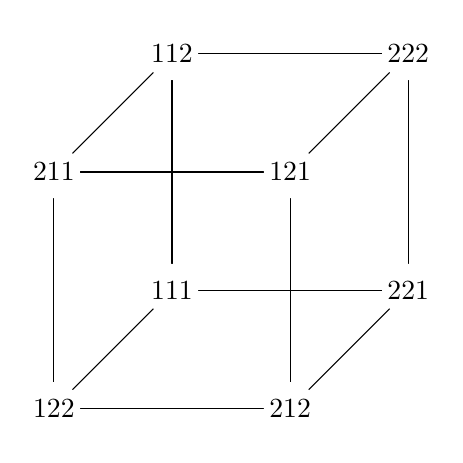
\begin{tikzpicture}[scale=1.5]
  % Priekinė siena
  \coordinate (A) at (0,0);
  \coordinate (B) at (2,0);
  \coordinate (C) at (2,2);
  \coordinate (D) at (0,2);
  % Galinė siena
  \coordinate (E) at (1,1);
  \coordinate (F) at (3,1);
  \coordinate (G) at (3,3);
  \coordinate (H) at (1,3);

  \draw (A) -- (B) -- (C) -- (D) -- cycle;
  \draw (A) -- (E);
  \draw (B) -- (F);
  \draw (C) -- (G);
  \draw (D) -- (H);
  \draw (E) -- (F) -- (G) -- (H) -- cycle;

  \node[circle, fill=white, inner sep=1pt] at (A) {122};
  \node[circle, fill=white, inner sep=1pt] at (B) {212};
  \node[circle, fill=white, inner sep=1pt] at (C) {121};
  \node[circle, fill=white, inner sep=1pt] at (D) {211};
  \node[circle, fill=white, inner sep=1pt] at (E) {111};
  \node[circle, fill=white, inner sep=1pt] at (F) {221};
  \node[circle, fill=white, inner sep=1pt] at (G) {222};
  \node[circle, fill=white, inner sep=1pt] at (H) {112};
\end{tikzpicture}
\end{center}


\begin{flushright}
Ats.: taip, gali.
\end{flushright}
 \vspace{6mm}  

%\vspace{0.3cm}
\hspace*{-5.2mm}
%\begin{minipage}[b][6cm][c]{0.5\textwidth}
\begin{minipage}{0.57\textwidth}
\begin{uzdavinys}
Plokštumoje duoti du vienas kito išorėje esantys ir bendrų taškų neturintys apskritimai $\mathcal S$ ir $\mathcal T$. Šiems apskritimams išvestos trys bendros liestinės bei pažymėti jų taškai, kaip parodyta paveikslėlyje ($A$ ir $B$ yra lietimosi taškai, $C$ ir $D$ yra liestinių susikirtimo taškai). Įrodykite, kad $AC=BD$.
\end{uzdavinys}
\end{minipage}\quad
%\begin{minipage}[t][1cm][t]{0.7\textwidth}
\begin{minipage}{0.8\textwidth}
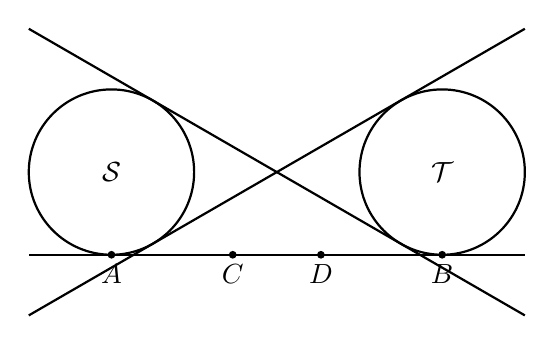
\begin{tikzpicture}[scale=0.7]
  \coordinate (S) at (0,0);
  \coordinate (T) at (6,0);
  
  \draw[thick] (S) circle (1.5);
  \draw[thick] (T) circle (1.5);
  
  % Apatinė bendra išorinė liestinė
  \draw[thick] (-1.5,-1.5) -- (7.5,-1.5);
  
  % Vidinės bendros liestinės
  % Apskaičiuojam vidinių liestinių sąlyčio taškus
  % R = 1.5, atstumas d = 6.
  % sin(alpha) = 1.5 / 3 = 0.5 -> alpha = 30 laipsnių
  
  % Liestinė iš viršaus kairės į apačią dešinę
  \coordinate (A) at ({1.5*cos(90+30)}, {1.5*sin(90+30)}); % = (-0.75, 1.3)
  \coordinate (H) at ({6+1.5*cos(270+30)}, {1.5*sin(270+30)}); % = (6.75, -1.3)
  \draw[thick] (-1.5, 2.6) -- (7.5, -2.6);
  
  % Liestinė iš apačios kairės į viršų dešinę
  \coordinate (E) at ({1.5*cos(270-30)}, {1.5*sin(270-30)});
  \coordinate (F) at ({6+1.5*cos(90-30)}, {1.5*sin(90-30)});
  \draw[thick] (-1.5, -2.6) -- (7.5, 2.6);
  
  % Pažymėti taškai (pagal užduoties logiką, šie taškai gali būti kitur, bet
  % pateikiu iliustracinį brėžinį, artimą originaliam).
  \coordinate (C) at (2.2, -1.5);
  \coordinate (D) at (3.8, -1.5);
  \coordinate (A_pt) at (0,-1.5);
  \coordinate (B_pt) at (6,-1.5);
  
  \fill (A_pt) circle (2pt) node[below] {$A$};
  \fill (B_pt) circle (2pt) node[below] {$B$};
  \fill (C) circle (2pt) node[below] {$C$};
  \fill (D) circle (2pt) node[below] {$D$};
  
  \node at (0, 0) {$\mathcal{S}$};
  \node at (6, 0) {$\mathcal{T}$};
\end{tikzpicture}
\end{minipage}
\vspace{0cm}

\textit{Sprendimas.} Tiesių ir apskritimų lietimosi taškus pažymėkime, kaip parodyta paveikslėlyje. Tiesių $EG$ ir $FH$ sankirtos tašką pažymėkime $O$.

\begin{center}
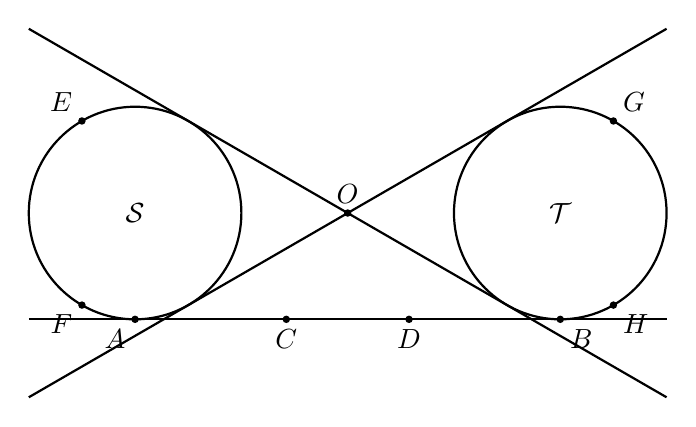
\begin{tikzpicture}[scale=0.9]
  \coordinate (S) at (0,0);
  \coordinate (T) at (6,0);
  
  \draw[thick] (S) circle (1.5);
  \draw[thick] (T) circle (1.5);
  
  % Apatinė liestinė
  \draw[thick] (-1.5,-1.5) -- (7.5,-1.5);
  
  % Vidinės liestinės (susikerta ties O(3,0))
  \draw[thick] (-1.5, 2.6) -- (7.5, -2.6);
  \draw[thick] (-1.5, -2.6) -- (7.5, 2.6);
  
  \coordinate (A) at (0,-1.5);
  \coordinate (B) at (6,-1.5);
  
  \coordinate (C) at ({3 - 1.5/tan(60)}, -1.5); % Intersection of left inner tangent and bottom tangent
  \coordinate (D) at ({3 + 1.5/tan(60)}, -1.5); % Intersection of right inner tangent and bottom tangent
  
  \coordinate (E) at ({1.5*cos(90+30)}, {1.5*sin(90+30)});
  \coordinate (F) at ({1.5*cos(270-30)}, {1.5*sin(270-30)});
  
  \coordinate (G) at ({6+1.5*cos(90-30)}, {1.5*sin(90-30)});
  \coordinate (H) at ({6+1.5*cos(270+30)}, {1.5*sin(270+30)});
  
  \coordinate (O) at (3,0);
  
  \fill (A) circle (1.5pt) node[below left] {$A$};
  \fill (B) circle (1.5pt) node[below right] {$B$};
  \fill (C) circle (1.5pt) node[below] {$C$};
  \fill (D) circle (1.5pt) node[below] {$D$};
  
  \fill (E) circle (1.5pt) node[above left] {$E$};
  \fill (F) circle (1.5pt) node[below left] {$F$};
  \fill (G) circle (1.5pt) node[above right] {$G$};
  \fill (H) circle (1.5pt) node[below right] {$H$};
  \fill (O) circle (1.5pt) node[above] {$O$};
  
  \node at (0, 0) {$\mathcal{S}$};
  \node at (6, 0) {$\mathcal{T}$};
\end{tikzpicture}
\end{center}

Šiame uždavinyje pakanka žinoti tokį geometrijos teiginį: jei dvi apskritimo liestinės kertasi taške $X$, o apskritimą liečia taškuose $Y$ ir $Z$, tai $XY=XZ$. Todėl:
\begin{itemize}
\item[1)] $CA=CE$ (apskritimas $\mathcal S$ ir jo liestinių sankirtos taškas $C$);
\item[2)] $DB=DH$ (apskritimas $\mathcal T$ ir taškas $D$);
\item[3)] $OE=OF$ (apskritimas $\mathcal S$ ir taškas $O$);
\item[4)] $OH=OG$ (apskritimas $\mathcal T$ ir taškas $O$);
\item[5)] $DA=DF$ (apskritimas $\mathcal S$ ir taškas $D$);
\item[6)] $CB=CG$ (apskritimas $\mathcal T$ ir taškas $C$).
\end{itemize}
Liko įvairiais būdais susieti šias lygybes. Pasinaudokime 3) ir 4): $$EG=OE+OG=OF+OH=HF.$$ Pasinaudokime 5) ir 6), o tada 1) ir 2):
 \begin{align*}AD-BC&=DF-CG=(DH+HF)-(CE+EG)=\\&=(DH-CE)+(HF-EG)=DH-CE=DB-CA.\end{align*}
Kita vertus, $$AD-BC=(AC+CD)-(BD+CD)=AC-BD.$$ Todėl $BD-AC\hm{=}AC-BD$, \,$2BD=2AC$\, ir \,$BD=AC$.

 \vspace{0,3cm}  

\begin{uzdavinys}
Išspręskite lygtį:
$$\frac{x^4+4}{x^2-2}=5x.$$
\end{uzdavinys}

\textit{Pirmasis sprendimas.} Galima padauginti abi lygties puses iš vardiklio $x^2-2$, bet tada turėsime ieškoti ketvirto laipsnio daugianario šaknų. Pertvarkykime lygtį kitaip. Pakeiskime skaitiklį, kad gautume reiškinį, besidalijantį iš vardiklio. Tam pastebėkime, kad $x^4+4$ ir $(x^2-2)^2=x^4-4x^2+4$ skiriasi per $4x^2$. Todėl
$$\frac{x^4+4}{x^2-2}=\frac{(x^4-4x^2+4)+4x^2}{x^2-2}=\frac{(x^2-2)^2}{x^2-2}+\frac{4x^2}{x^2-2}=x^2-2+\frac{4x^2}{x^2-2}.$$
Gauname pertvarkytą lygtį $$x^2-2+\frac{4x^2}{x^2-2}=5x.$$ Pastebėkime dar vieną dėsningumą: padaliję jos abi puses iš $x$, gausime panašius reiškinius $\frac{x^2-2}x$ ir $\frac x{x^2-2}$. Dalyti iš~$x$ galime, nes $x=0$ netenkina duotosios lygties, o padaliję gauname
$$\frac{x^2-2}{x}+\frac{4x}{x^2-2}=5,\text{~ arba ~}t+\frac{4}{t}=5,\text{ kur }t=\frac{x^2-2}{x}.$$
Padauginę gautąją lygtį iš $t$, turime nebe ketvirto laipsnio, o nesudėtingą kvadratinę lygtį $t^2-5t+4=0.$
Taigi $\frac{x^2-2}{x}=t=1$ arba 4. Tada $x^2-x-2=0$ arba $x^2-4x-2=0$. Šių lygčių sprendiniai yra $x_1=-1$, $x_2=2$, $x_{3,4}=2\pm\sqrt{6}$.

Visi keturi sprendiniai tenkina duotąją lygtį. Pavyzdžiui, $x_3^2=\left(2+\sqrt{6}\right)^2=10+4\sqrt{6}$, \begin{align*}\frac{x_3^4+4}{x_3^2-2}&=\frac{\left(10+4\sqrt{6}\right)^2+4}{10+4\sqrt{6}-2}=\frac{200+80\sqrt{6}}{8+4\sqrt{6}}=\frac{50+20\sqrt{6}}{2+\sqrt{6}}=\\&=\frac{\left(50+20\sqrt{6}\right)\left(2-\sqrt{6}\right)}{\left(2+\sqrt{6}\right)\left(2-\sqrt{6}\right)}=\frac{-20-10\sqrt{6}}{4-6}=10+5\sqrt{6}=5x_3.\end{align*}

 \vspace{0,3cm} 
 
 \textit{Antrasis sprendimas.} Pertvarkę $x^4+4=5x(x^2-2)$, gauname lygtį
 $p(x)=0,$ kur~$p(x)$ yra ketvirto laipsnio daugianaris $$x^4-5x^3+10x+4.$$ Spėliojant lengva rasti jo šaknis $-1$ ir 2 (tai yra ir duotosios lygties sprendiniai). Daugianaris su tokiomis šaknimis dalijasi iš $x-(-1)$ ir $x-2$, t.~y.
 $p(x)=(x+1)(x-2)q(x)\hm=(x^2-x-2)q(x),$ kur $q(x)$ yra daugianaris. Jį galima rasti pertvarkant $p(x)$:\begin{align*}p(x)&=x^2(x^2-x-2)-4x^3+2x^2+10x+4=\\&=
 x^2(x^2-x-2)-4x(x^2-x-2)-(2x^2-2x-4)=\\&=(x^2-x-2)(x^2-4x-2).\end{align*} Taigi $p(x)=0$ reiškia, kad $x^2-x-2=0$ arba $x^2-4x-2=0$. Liko išspręsti šias dvi lygtis ir patikrinti gautus sprendinius kaip pirmajame sprendime.

\begin{flushright}
Ats.: $x=-1$, \,2 arba $2\pm\sqrt{6}$.
\end{flushright}
 \vspace{0,7cm}

\begin{center}\label{dvu}
{\sc\large 2008 m.~10 klasės uždavinių (Vilniaus m.) sprendimai}
\end{center}
\vspace{0,3cm}


\setcounter{uzdavinys}{0}


\begin{uzdavinys}
Ant stalo stovi 13 neuždegtų lempų, kiekviena su savo jungikliu, kuris nedegančią lempą uždega, o degančią užgesina.
\begin{itemize}
\item[a)] Vienu ėjimu galima nuspausti bet kuriuos 8 jungiklius. Ar taip elgiantis galima pasiekti, kad visos lempos degtų vienu metu?
\item[b)] Vienu ėjimu galima nuspausti bet kuriuos 7 jungiklius. Ar taip elgiantis galima pasiekti, kad visos lempos degtų vienu metu?
\end{itemize}
\end{uzdavinys}

\textit{Sprendimas.}\footnote{Taip pat žr.~panašų 9 klasės 1 uždavinį ir jo sprendimą.} a) Priskirkime kiekvienai lempai skaičių: 0, jei ji nedega, ir 1, jei dega. Pradžioje turime 13 nulių. Kiekvienu ėjimu mes pakeičiame 8 skaičius: $x$ vienetų ($0\leq x\leq8$) pakeičiame nuliais ir $8-x$ nulių pakeičiame vienetais. Visų 13 skaičių suma sumažėja~$x$ vienetų ir padidėja $8-x$ vienetų. Taigi ji padidėja $(-x)+(8-x)=2(4-x)$ vienetų, t.~y.~lyginiu skaičiumi. Vadinasi, sumos lyginumas nepakinta. Pradžioje suma lygi~0. Ji lyginė, todėl ir liks lyginė, kiek ėjimų beatliktume.

Niekada negausime situacijos, kai visos lempos dega, nes šioje situacijoje visi skaičiai būtų vienetai ir jų suma 13 būtų nelyginė.
%\vspace{0,3cm}

b) Įsivaizduokime lempas stovint ratu ir iš eilės sunumeruokime jas skaičiais nuo 1 iki~13. Apeidami pilną ratą nagrinėkime gretimų lempų septynetus (1, 2, 3, 4, 5,~6,~7), (2,~3, 4, 5, 6, 7, 8), $\ldots$, (12, 13, 1, 2, 3, 4, 5), (13, 1, 2, 3, 4, 5, 6) (tokių septynetų yra~13) ir pakeiskime lempų būsenas iš eilės kiekviename iš jų. Kiekviena lempa priklauso~7 septynetams, todėl jos būsena pakinta 7 kartus. Taigi kiekvienos lempos būsena pakeičiama priešinga, t.~y.~visos lempos uždegamos.

\begin{flushright}
     Ats.: a) negalima; b) galima.
\end{flushright}
 \vspace{0,6cm}  

\hspace*{-5.2mm}
\begin{minipage}%[b][6cm][c]
{0.78\textwidth}
\begin{uzdavinys}
Stačiojo trikampio $ABC$ įžambinėje $AB$ taip pažymėti taškai $M$ ir $N$, kad $AN=AC$ ir $BM=BC$ (žr.~pav.). Tada statiniuose $BC$ ir~$AC$ atitinkamai pažymėti tokie taškai $P$ ir~$Q$, kad $BP=BN$ ir $AQ=AM$. Įrodykite, kad taškai $C$, $P$, $N$, $M$ ir $Q$ priklauso vienam apskritimui.
\end{uzdavinys}
\end{minipage}\quad%\qquad
\begin{minipage}%[b][6cm][c]
{0.8\textwidth}
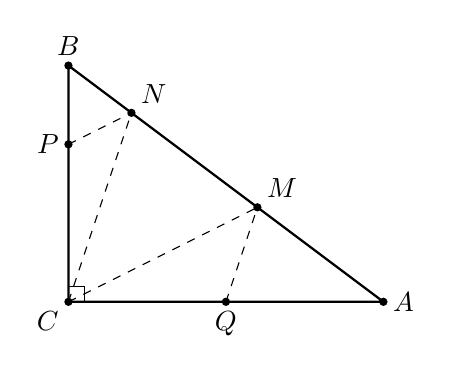
\begin{tikzpicture}[scale=1]
  \coordinate (C) at (0,0);
  \coordinate (A) at (4,0);
  \coordinate (B) at (0,3);

  \draw[thick] (C) -- (A) -- (B) -- cycle;
  \draw (C) rectangle (0.2,0.2);

  % AN = AC = 4
  \coordinate (N) at ($(A)!4/5!(B)$); 
  % BM = BC = 3
  \coordinate (M) at ($(B)!3/5!(A)$);

  % AQ = AM = 5-3 = 2
  \coordinate (Q) at ($(A)!2/4!(C)$);
  % BP = BN = 5-4 = 1
  \coordinate (P) at ($(B)!1/3!(C)$);

  \draw[dashed] (C) -- (M);
  \draw[dashed] (C) -- (N);
  \draw[dashed] (Q) -- (M);
  \draw[dashed] (P) -- (N);

  \foreach \p in {A,B,C,M,N,P,Q} \fill (\p) circle (1.5pt);

  \node[right] at (A) {$A$};
  \node[above] at (B) {$B$};
  \node[below left] at (C) {$C$};
  \node[above right] at (M) {$M$};
  \node[above right] at (N) {$N$};
  \node[left] at (P) {$P$};
  \node[below] at (Q) {$Q$};
\end{tikzpicture}
\end{minipage}
\vspace{0cm}


\textit{Sprendimas.}  Trikampiai $QAM$ ir $CAN$ yra lygiašoniai ($AQ=AM$ ir $AC=AN$) ir turi bendrą kampą, esantį prieš pagrindą, todėl ir jų kampai prie pagrindo yra visi lygūs tarpusavyje (jie lygūs $\frac{180^\circ-\angle A}2$). Taigi $\angle CNM+\angle CQM=\angle CNM\hm+(180^\circ-\angle MQA)\hm=180^\circ.$ Kadangi priešingų keturkampio $CQMN$ kampų suma lygi $180^\circ$, tai jis įbrėžtinis, t.~y. taškas $Q$ priklauso apskritimui per $C$, $M$, $N$. (Beje, galima pastebėti, kad $CQMN$ yra lygiašonė trapecija, o lygiašonė trapecija visada yra įbrėžtinis keturkampis.)

Analogiškai įrodoma, kad $P$ priklauso apskritimui per $C$, $M$, $N$. Vienintelis apskritimas, einantis per tris taškus $C$, $M$ ir $N$, eina ir per taškus $P$ bei $Q$. Vadinasi, taškai $C$, $P$, $N$, $M$ ir $Q$ priklauso vienam apskritimui.

 \vspace{0,3cm}  

\begin{uzdavinys} 
Tegu $x$ yra dešimties iš eilės einančių natūraliųjų skaičių suma, o $y$ -- tų pačių dešimties skaičių kubų suma. Įrodykite, kad $y^2-x^2$ dalijasi iš 12.
\end{uzdavinys}

\textit{Sprendimas.}\footnote{Taip pat žr.~panašų 12 klasės 3 uždavinį ir jo sprendimą.} Mažiausią iš 10 natūraliųjų skaičių pažymėkime $n$. Tada \begin{align*}y-x&=(n^3+(n+1)^3+\ldots+(n+9)^3)-(n+(n+1)+\ldots+(n+9))=\\&=(n^3-n)+((n+1)^3-(n+1))+\ldots+((n+9)^3-(n+9)).\end{align*}
Kiekvieną iš 10 gautų dėmenų galima užrašyti kitaip: $$m^3-m=m(m^2-1)=(m-1)m(m+1),\text{ kai }m=n, \,n+1, \,\ldots, \,n+9.$$ Taigi kiekvienas dėmuo yra trijų gretimų sveikųjų skaičių sandauga. Tarp trijų gretimų sveikųjų skaičių visada yra vienas, dalus iš 3, ir bent vienas, dalus iš 2. Todėl tiek visi dėmenys, tiek jų suma $x-y$ dalijasi iš $2\cdot3=6$. Kadangi $x-y$ dalijasi iš 2, tai $x+y\hm=(x-y)+2y$ taip pat dalijasi iš 2. Vadinasi, skaičius $x^2-y^2=(x-y)(x+y)$ dalijasi iš $6\cdot2=12$.

 \vspace{0,3cm}  


\begin{uzdavinys}
Duota kvadratinė lentelė, sudaryta iš $4\times4$ vienetinių langelių. Kai kurie langeliai nudažyti taip, kad vienu metu išbraukus bet kurias dvi eilutes ir bet kuriuos du stulpelius, gautoje $2\times2$ lentelėje lieka bent vienas nudažytas langelis. Kiek mažiausiai langelių nudažyta?
\end{uzdavinys}

\textit{Sprendimas.}\footnote{Panašiai galima išspręsti analogišką uždavinį apie $2n\times2n$ lentelę kiekvienam natūraliajam $n$: žr.~12 klasės 4 uždavinį ir jo sprendimą. Taip pat žr.~panašų 11 klasės 4 uždavinį ir jo sprendimą.} Uždavinio sąlygoje nurodytą lentelės nudažymo savybę paranku performuluoti taip: bet kurių dviejų stulpelių nudažytieji langeliai yra išsibarstę bent per tris eilutes. Perrenkant visas stulpelių poras, galima greitai patikrinti, kad šia savybe pasižymi nudažymas, parodytas paveikslėlyje. Vadinasi, lentelėje gali būti nudažyti tik~7 langeliai.

\begin{center}
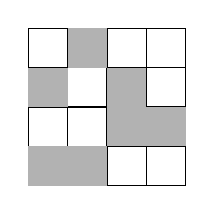
\begin{tikzpicture}[scale=0.5]
  \draw (0,0) grid (4,4);
  \fill[black!30] (0,0) rectangle (1,1);
  \fill[black!30] (1,0) rectangle (2,1);
  \fill[black!30] (2,1) rectangle (3,2);
  \fill[black!30] (3,1) rectangle (4,2);
  \fill[black!30] (0,2) rectangle (1,3);
  \fill[black!30] (2,2) rectangle (3,3);
  \fill[black!30] (1,3) rectangle (2,4);
\end{tikzpicture}
\end{center}

Kita vertus, galima įrodyti, kad lentelėje negali būti mažiau nei 7 nudažyti langeliai. Tam pastebėkime, kad bet kuriuose dviejuose stulpeliuose turi būti bent trys nudažyti langeliai (esantys skirtingose eilutėse), ir išskirkime tris atvejus:
\begin{itemize}
\item[1)] lentelėje yra stulpelis be nudažytų langelių; tada kiekviename iš likusių stulpelių yra bent po tris nudažytus langelius, o iš viso yra bent $3\cdot3=9$ nudažyti langeliai; 
\item[2)] lentelėje yra stulpelis su lygiai vienu nudažytu langeliu; tada kiekviename iš likusių stulpelių yra bent po du nudažytus langelius, o iš viso yra bent $1+3\cdot2=7$ nudažyti langeliai;
\item[3)] kiekviename stulpelyje yra bent du nudažyti langeliai; tada iš viso yra bent $4\cdot2=8$ nudažyti langeliai.
\end{itemize}
Visais trimis atvejais nudažytų langelių skaičius yra ne mažesnis nei 7. 

Vadinasi, mažiausias galimas nudažytų langelių skaičius yra 7. 


\begin{flushright}
Ats.: 7.
\end{flushright}
 \vspace{0,7cm}  
%\newpage


\end{document}